\section{Why don't we Understand the News?}

The day the result of the 2016 United Kingdom EU Membership Referendum was announced, the \citeauthor{googletrends} reported a 250\% increase in searches for ``What happens if we leave the EU?''. Much like the case of David Leonhardt's 2008 article in the New York Times in which began, ``Raise your hand if you don't quite understand this whole financial crisis,'' national news commentary had focused on little else in the preceding months.

Some months after Leonhardt's article was published, Journalism Professor Jay Rosen voiced his agreement with its premise in a blog post on the failure of journalism during the financial crisis; ``there are certain very important stories -- and the mortgage crisis is a good example -- where until I grasp the whole I am unable to make sense of any part.''\citep{NationalExplainer} 

It has become apparent that prolific coverage alone is not enough to engage and support the public in understanding the complexities of current events. Historically, news media has been limited in the volume of content it can produce by physical constraints such as printing costs, but the rise of the internet as a platform to deliver it has lead to an explosion of content, both through existing media channels and through competing social media websites and blogs. 

The term \textit{ambient news} was coined by \citet{newnewsoldnews} to describe the ubiquity of news in the current information landscape. Others have commented in a more critical light; describing the proliferation of competing news media as ``as pervasive--and in some ways as invasive--as advertising.'' \citep[p.2]{overloadjournalismsbattle}


In 2007, The Associated Press conducted an extensive field study \citeyear{anewmodelfornews} into the news consumption habits of young adults. Among their key findings were three points which essentially summarise the news overload issue;
\begin{itemize}
	\item \textbf{``Consumers are experiencing news fatigue.''} \par
	The study found participants were debilitated, and that their levels of dissatisfaction lead to a decrease in the effort they put into news acquisition. This is consistent with multiple other studies \citep{newsandtheoverloadedcustomer, UnderstandingTheParticipatoryNewsConsumer, InformationAccessinComplexPoorlyStructuredInformationSpaces} which found participants across every demographic were overwhelmed by the amount of news content available to them and agreed it prevented them exploring news on less familiar topics. 
	
	\item \textbf{``Story resolution is key.''} \par
	Participants' consistent enjoyment of sports and entertainment news was due in part to the formulaic storytelling which characterises these types of journalism, with clear chronology to provide contextual back story. The feeling of enjoyment gained from reading procedural stories directly contrasts with what the same participants experienced reading World news, where they struggled to find resolution to stories which were unfolding at the time.
	
	\item \textbf{``Consumers want depth but aren't getting it''} \par
	It was observed that participants, in their efforts to discover \textit{below-the-fold} content (defined in the context of the AP's model, \citeyear[p.37]{anewmodelfornews}) from particular headlines, often found themselves reading the same summary-level content from different news sources. It was recommended that news providers support this by ``designing innovative formats and creating easier pathways to deep content.'' \citep[p.49]{anewmodelfornews}
\end{itemize}

Initially, the third point seems to be a direct contradiction to the first; we are overwhelmed by the volume of news we are exposed to, but we also crave more detail from the news we do consume. However, it brings to light the issue of information \textit{quality} as a requirement of news consumers.

 Journalism, and therefore its quality, can be viewed along a spectrum between two models; a model for the communication of facts, and a model for entertainment and storytelling. From the three points above, it is clear that quality at both ends of the spectrum is being sought, since the desire for quality below-the-fold content is covered by the first model, and the desire for quality story resolution by the second.

\subsection{Information Overload \label{sec:information-overload}}

News fatigue is a domain-specific type of information overload, a phenomenon formally defined as ``when the information processing demands on time to perform interactions and internal calculations exceed the supply or capacity of time available for such processing'' \citep[p.206]{InformationOverloadATemporalApproach}. Information overload is a multifaceted problem which can be modelled as a combination of three contributing factors (Figure \ref{fig:dimensions}).

\begin{figure}[htbp!]
	\centering
	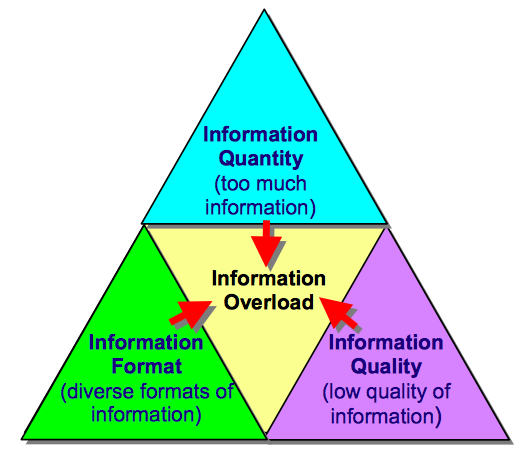
\includegraphics[width=.6\textwidth]{img/lit-survey/overload-model.png}
	\caption{Dimensions of information overload, as defined by \citet{TowardsAnOptimalResolutionToInformationOverload}.}
	\label{fig:dimensions}
\end{figure}

These factors correspond directly to the three points previously identified from the \citeauthor{anewmodelfornews} study. High information quantity leads to news fatigue, information format determines the level of possible story resolution, and information quality determines how much depth a reader can gain from the news they consume. The authors did not find a single solution which could address all three factors, but they did identify information quantity as the most significant contributor to overload.

\citet{GuestEditorsIntroductionInformationOverload} further decompose information quantity into spatial and temporal dimensions in the specific context of news articles. Spatial quantity refers to articles which are near-identical in terms of facts presented being published by different media outlets, and temporal quantity refers to articles on a single topic being published in quick succession over a short period of time. 

Intuitively, the terms spatial and temporal quality seem illogically named, as a set of articles with high spatial quantity would cover a smaller area of information space and vice versa. High spatial quantity will therefore be refered to as \textit{redundancy}, and high temporal quantity as \textit{fragmentation}, since a sudden burst of articles published on the same topic suggests a currently unfolding story being told in parts.

To adequately determine the contributory factors relating to news fatigue, all four dimensions of information overload should be considered, and will therefore be explored in more detail in the following sections.

\subsubsection{Information Format}
The domain of news articles is a more specific information space than that of documents in general, and by nature most news articles share some common formatting and structural elements such as headlines, timestamps, and relevant images. As a result of this, it is unlikely that any two articles from popular news providers would be diverse enough in content format to overshadow the information quantity problem.

\subsubsection{Information Quality}
In the context of factual data rather than news specifically, \citet{DataQualityInContext} defined information quality in terms of four components; intrinsic quality, accessibility quality, contextual quality and representational quality. If news can be rationalised to its core function as an interpretation of facts and other raw data such as images, then this same framework can be experimentally applied to news journalism in order to determine which factors could influence its quality.

Intrinsic quality is a measure of the accuracy, objectivity, believability and reputation of data. In the context of news, the first three factors would typically be true for all major news sources, and the reputation would be dependent on whether the article originated from a trusted source or not. Accessibility quality is less relevant to online news media, as it is concerned with data access and security. Contextual quality is the most relevant category in respect to news, concerning timeliness, amount of data, and value-added. In the news domain, this would mean an article's quality is dependent on its performance against a background of other articles; whether or not it contributes anything recent or previously unknown. Finally, representational quality is concerned with ease of understanding and interpretability, which are easily translatable concepts.

To summarise, applying the Information Quality Framework \citep{DataQualityInContext} to news articles suggest quality can be influenced by the reputation of the source, the timeliness of publication, value-added by the article (i.e. content which couldn't be derived from other sources) and ease of understanding.

\subsubsection{Fragmentation (Temporal Quantity)}

The rise of social media sites such as Twitter delivering news to consumers has lead to a high degree of news fragmentation, due to the constraints of the microblogging service's 140-character limit. 24-hour television news paved the way for new formats of real-time content delivery, and the ever-expanding network of online social media channels stepped up to deliver. 

It logically follows from the fragmented nature of real-time news journalism that temporal quality suffers; stories are published and updated intermittently over short periods of time, meaning there is more content for the consumer to piece together in order to understand a story. The fragmentation is somewhat mitigated by Twitter's use of hashtags to denote a Tweet's topics. Hashtags help readers form a coherent and picture of unfolding events from the incremental contributions of thousands of participating users \citep{BlogsTwitterAndBreakingNews}.

\citet{BreakingNewsDetectionAndTrackingInTwitter} developed a methodology to collect and group Tweets on breaking news topics, using hashtags for topic identification or \textit{story-finding}, and grouping similar messages together to form a single news story. Their algorithm for similarity is a function of the TF-IDF \citep{TermWeightingApproachesInAutomaticTextRetrieval} of the two messages and the number of named entities they have in common.

\subsubsection{Redundancy (Spatial Quantity)}
It is in the nature of news that newsworthy stories get repeated across multiple sources. When consumers read news on a particular from more than once source, it is likely that they will read variations on the same facts in multiple articles.

Attempts such as \citep{InformationFusionInTheContextOfMultiDocumentSummarization} have been made to synthesise summaries of collections of similar online documents, a practice here termed \textit{information fusion}, with news articles from different sources being given as a specific use-case. However, the process of extracting common sentences between documents was in order to reformulate them into a single summary, rather than to determine the level of similarity between the documents.

A more relevant approach was presented in \citep{UtilizingPhraseSimilarityMeasures}, where the \textit{title} and \textit{description} attributes of elements in RSS feeds were used as content descriptors to mitigate the overhead of processing entire documents for phrases. The content descriptors are then used to compute phrase \textit{n}-grams as a measure of similarity between any two documents. The similarities in this case were used to remove subsumed articles and cluster non-redundant similar ones, in order to streamline feed content for readers.

It should be noted that there is an overlap between the notion of spatial quantity and one of the four influencing factors in information quality; contextual quality. If a feed contains two articles which state the same number of identical facts, they therefore contribute to information overload on both the qualitative and quantitative fronts.

Viewing the dimensions of overload from a news domain perspective, it is clear that (consistent with the findings of \citet{TowardsAnOptimalResolutionToInformationOverload}) information quantity is the most relevant contributing factor in respect to fatigue, along factors influencing contextual quality such as value-added and timeliness. Any proposed solutions to the news overload problem should therefore address these factors first.

\subsection{Supporting Sensemaking}

Sensemaking is the basis for forming contextual knowledge; the process by which we incorporate new information into our existing cognitive frameworks, and how we go from reading something to understanding it \citep{FromInformationToKnowing}. In broader terms, \citeauthor{OrganizingAndTheProcessOfSensemaking} describe sensemaking as ``[being] about the question: What does an event mean? In the context of everyday life, when people confront something unintelligible and ask, `What's the story here?'{}'' \citep[p.85]{OrganizingAndTheProcessOfSensemaking} 

This definition relates directly to the news overload problem because sensemaking describes the contextual story resolution the \citet{anewmodelfornews} study identified news consumers are craving. It has also been observed that often readers are not interested in specific articles on a subject, and only the thematic content of the topic they belong to \citep{AnalysingUserAccessToAnOnlineNewspaper}. How then, do readers make sense of a collection of articles surrounding a particular topic?

When presented with a large document collection, \citet{BeingLiteratreWithLargeDocumentCollections} found all of their subjects began by clustering the contents into groups which formed a heuristic representation or mental model, used to provide an overview. However, current information infrastructure has been criticised for not supporting the cross-correlation between connected news articles \citep{GalaxyOfNews}.

Writing for the Columbia Journalism review in 2008, \citeauthor{overloadjournalismsbattle} outlined a suggestion for the new roles of journalism in the information era; ``By linking stories to one another and to background information and analysis, news organizations help news consumers find their way through a flood of information that without such mediation could be overwhelming and nearly meaningless.''\citep[p.10]{overloadjournalismsbattle} 

Similarly, \citet{FromInformationToKnowing} make the recommendation in the context of contemporary media consumption that news providers should adapt to an environment of news overload by adding facilities enabling readers to categorise, sort and search news collections. Additional findings of this study suggested that the contextual background provided by having more detailed coverage aids the sensemaking process, as it helps users form links between new information and their existing frameworks, but this presents an interesting conflict with the goal of reducing information overload when considering large collections of documents.

In summary, many recommendations have been made from within the field of journalism that at the point of delivery, news content should incorporate contextual links to related articles. This is important both from a sensemaking perspective to emphasise connections, and from an information overload perspective to help users find meaning in an inundated news landscape.

The news overload problem can now be reformulated with scope and detail: How can we display a collection of related news articles in such a way that users are not overwhelmed by unstructured content and are free to explore the underlying contextual pathways?

A simple starting point comes from a familiar idiom; a picture is worth a thousand words.

\section{An Overview of Information Visualisation}

Of course, a picture is not always worth a thousand words, particularly when the picture is unstructured and complex in its own right. However, a recognised and effective technique for bridging the gap between a set of data and a user's mental model and subsequent comprension of the data is information visualisation, or InfoVis. \citep{UnderstandingAndCharacterizingInsights, ThemeRiver}. This section provides a brief overview of a formative InfoVis taxonomy and uses the taxonomy to categorise appropriate visual models for news feed visualisation.

In his seminal paper on information visualisation, \citeauthor{TheEyesHaveIt} proposed a taxonomy for visualisations comprising seven data type abstractions, and seven tasks which are components of the visual information seeking mantra; ``Overview first, zoom and filter, then details-on-demand.'' \citep[p.1]{TheEyesHaveIt}

\citeauthor{TheEyesHaveIt}'s type abstractions are as follows:
\begin{description}[leftmargin=11em,style=nextline]
	\item [1-dimensional] Linear data, e.g. documents, where each datum is a string of characters.
	\item[2-dimensional] Planar data, e.g. cartographs, layout diagrams, or spatially-clustered document collections.
	\item[3-dimensional] Physical objects or models of real-world entities, e.g. computer aided designs or medical imaging data.
	\item[Multi-dimensional] Any data where items with n attributes can be represented in n-dimensional space, e.g. relational databases, or feature vectors for classification.
	\item[Temporal] Data following a timeline, which is a subset of 1-dimensional data but was deemed important enough to warrant its own category. E.g. Project management data, or multimedia content timelines.
	\item[Tree] Hierarchical data where each datum has exactly one parent and zero or many children, e.g. document or directory structures.
	\item[Network] Related data, where each datum can have an arbitrary number of links to other data.
\end{description}

Because of the non-spatial nature of textual data, any visualisation of such data must involve some form of content abstraction and translation into a physical space \citep{VisualizingTheNonVisual}. These translations can result in data of arbitrary dimensionality, so a text corpus could fall into the 1-dimensional or multi-dimensional categories. News articles as a specific subset of textual data have certain metadata associated with them including dates, meaning they also fit the temporal type abstraction. In addition to this, if contextual links are considered part of the structure of the data, articles can be modelled as a network of connected nodes.

This ambiguity is not a failure of the taxonomy; \citeauthor{TheEyesHaveIt} stresses that composite categories are equally valid. However, the implications of this are that the most appropriate visualisation for a news corpus may itself be a composite of visualisations for any of its type abstractions, leaving an unfeasible number of possibilities to consider. 

To reduce the scope of suitable visualisations, we return to the original problem of information overload. This time however, the aim is to minimise the overload from interpreting the model, rather than the overload from interpreting the data. Complex visualisations which require a considerable amount of effort to understand in their own right should be avoided where possible when reducing overload is the goal.

\subsection{InfoVis for Sensemaking}

In addition to the insight that visualisation may be able to provide, there is evidence that visual representation metaphors also focus users' attention, support the learning process, and utilise memory more effectively than isomorphic text representations \citep{LearningFromArchitects}.

\citet{UnderstandingAndCharacterizingInsights} identified four overlapping InfoVis processes which describe how insight can be gained after sensemaking; \textit{Provide Overview}, \textit{Adjust}, \textit{Detect Pattern}, and \textit{Match Mental Model}. These four processes can be roughly mapped to \citeauthor{TheEyesHaveIt}'s high-level tasks, which are as follows:

\begin{description}[leftmargin=11em,style=nextline]
	\item [Overview] Gain a birds-eye view of the entire collection, with the option to change the scale of the view by zooming or using fisheye magnification techniques.
	\item[Zoom] Gain a more detailed view of a portion of data or single datum while preserving the original sense of context.
	\item[Filter] Nondestructively remove uninteresting data points or groups from the view.
	\item[Details-on-Demand] Gain additional insight into one or more data points by selecting particular elements.
	\item[Relate] View and explore relationships between elements.
	\item[History] If necessary, undo previous actions to return to the a view of the data.
	\item[Extract] Export selected data, preserving the format, for uses such as ``sending by email, printing, graphing, or insertion into a statistical or presentation package.'' \citep[p.5]{TheEyesHaveIt}
\end{description}

The \textit{Provide Overview} process allows a reader to recognise what they know and what they don't know from the information they are processing. The corresponding task in \citep{TheEyesHaveIt} is \textit{Overview}.

\textit{Adjust} allows them to change the level of abstraction or field of selection of that information. This corresponds to \textit{Zoom} and \textit{Filter} in \citeauthor{TheEyesHaveIt}'s task model.

The \textit{Detect Pattern} procedure is where structure and trends are found (whether expected or otherwise). Coupled with \textit{Match Mental Model}, where the links are formed between the new data and the users' existing cognitive frameworks, this corresponds to \textit{Relate}.

At this point, \citeauthor{TheEyesHaveIt}'s taxonomy diverges from \citeauthor{UnderstandingAndCharacterizingInsights}, are \citeauthor{UnderstandingAndCharacterizingInsights} is concerned with the cognition enabled by visualisation, whereas  \citeauthor{TheEyesHaveIt} additionally considers other use cases for visualisations, such as querying and sharing.

From these two models, it is apparent that certain views and functions are crucial for tools which use visualisation to support the sensemaking process; an high-level overview visualisation which emphasises links between data, the ability to adjust scope to show more or less detail, and the ability to filter information of specific interest within the dataset.

\subsection{Visual Metaphors}

The use of preexisting visual metaphors--specifically those with which a large number of people will already be familiar--has been shown to support readers' comprehension, as it requires both significant time and effort for a reader to interpret visual metaphors which are new to them \citep{PreconceptionsVisualMetaphors}.

\citeauthor{AComparisonBetweenConceptMaps} defines visual metaphors as ``a graphic structure that uses the shape and elements of a familiar natural or man-made artefact or of an easily recognizable activity or story to organize content meaningfully and use the associations with the metaphor to convey additional meaning about the content.'' \citep[p.203]{AComparisonBetweenConceptMaps} 

Examples of visual metaphors commonly used to represent collections of data include calendars, bookshelves, timelines and maps. These do not have to be visually skeuomorphic to be effective, but to avoid misinterpretation, there should be a match between the underlying structure of the metaphor and the underlying structure of the data.

\subsubsection{Timelines}

Chronological ordering is an important characteristic of news articles and should be preserved in any visualisation of news data as it provides a natural ordering \citep{StructuredSummarizationForNewsEvents}. Perhaps the simplest visual metaphor for a collection of dated documents is the timeline.

\citeauthor{SchemaLine} explore the role of timelines in the sensemaking process,  emphasising that the interactions supported by such visualisations should be as intuitive as possible in order to not disrupt users' trains of thought, and should be tightly coupled with other elements of the sensemaking process so temporal connections are not viewed solely in isolation.

Criticisms of previous timeline visualisations made by the authors are that linear layouts  are often too simple for the data they represent, and that a lack of automatic layout generation results in additional manual work for the user \citep{SchemaLine}.

The colouring technique used to distinguish sets of related events within a single timeline is a flexible extension to \citep{TimeSets}, where the authors coloured events belonging to multiple sets with a gradient composed of the colours of both sets. 

The gradient approach does not scale to events belonging to more than two sets, and the colour grouping restricts the number of possible intersections of each set. From a news storyline perspective, this would place an upper limit of two on the number of possible topics a story could belong to, which is an impractical constraint.

\citet{ExploringLongRunningNewsStoriesUsingWikipedia} designed a prototype for generating annotated timelines based on the Wikipedia entries long-running news stories. The use of Wikipedia rather than news feeds meant their document retrieval model was heavily dependent on Wikipedia's structure, but it also afforded a huge wealth of contextual information that made such detailed annotations possible. Not all stories are long running however, so while this would be useful as a retrospective tool it would be impossible to generate timelines in the same way for news articles which did not already belong to a long-running chain of events.

Both ESTHETE \citep{ESTHETE} and nReader \citep{Nreader} present timeline-centric views for collections of news articles based on underlying graphs of relationships between the articles. However, in both cases, the graph structure was not part of the final visualisation, so connections between entities were displayed in purely textual forms.

In contrast, ThemeRiver \citep{ThemeRiver} introduces a novel view on topic frequency along the time axis to show thematic change over time within a collection of documents, similar to a smoothed histogram. This view, while useful for large document collections which span weeks or months, would be less suited to displaying emerging news trends over shorter periods of time.

\begin{figure}[h]
\centering
\begin{minipage}{.45\textwidth}
  \centering
  \hspace{-1cm}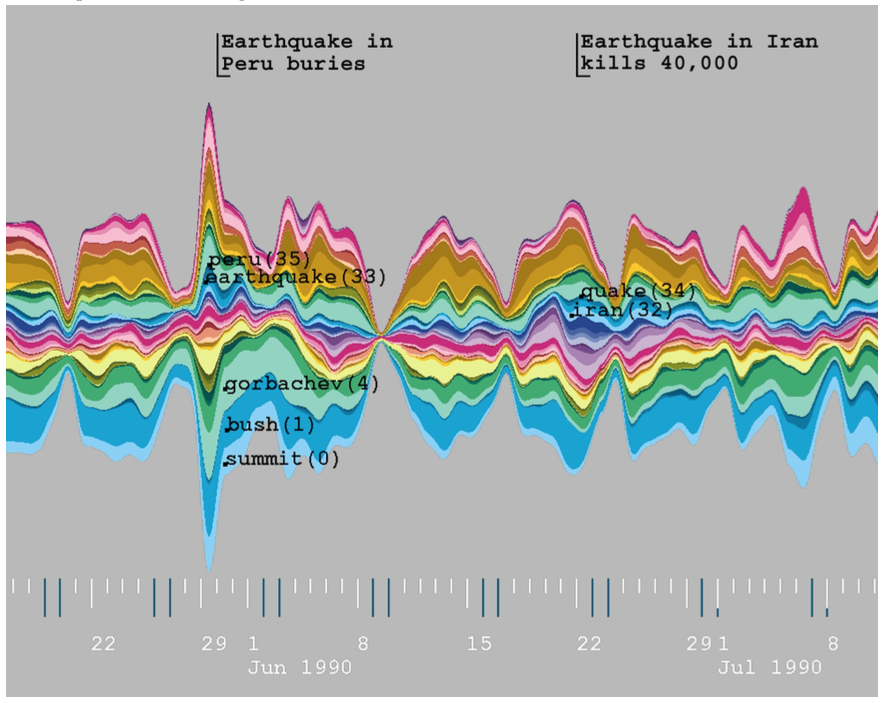
\includegraphics[width=.9\linewidth]{img/lit-survey/histogram1.png}
  \end{minipage}%
\begin{minipage}{.65\textwidth}
  \centering
  \hspace{-1.5cm}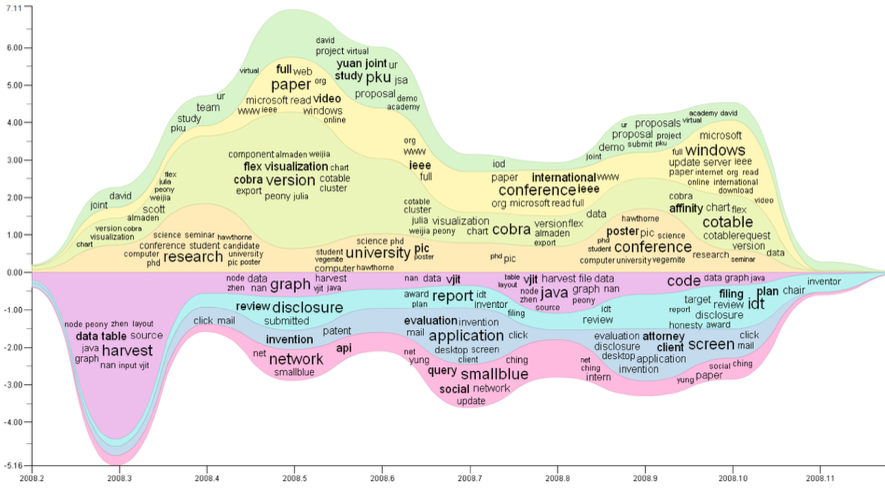
\includegraphics[width=.9\linewidth]{img/lit-survey/histogram2.png}
\end{minipage}
\caption{Similar visualisations from ThemeRiver \citep{ThemeRiver} (left) and TIARA \citep{InteractiveTopicBasedVisualTextSummarizationAndAnalysis} (right).}
  \label{fig:themeriver-tiara}

\end{figure}

TIARA \citep{InteractiveTopicBasedVisualTextSummarizationAndAnalysis} which cites ThemeRiver as an influencing design (see figure \ref{fig:themeriver-tiara}), displays a similar shaped graphical output but performs more detailed textual analysis, and displays related keywords in the output. Both visualisations support simple zooming and panning, but suffer from the same limitations on visualising topic connectivity as \citep{TimeSets}.

Taking into consideration both the critiques of  oversimplification identified in \citep{SchemaLine} and the physical limitations highlighted in \citep{TimeSets, ThemeRiver}, it is clear that timelines may not be the most appropriate visual metaphor for news visualisation, especially not for highly connected events and topics. 

However, for more linear storylines in which span fewer categories or topics, a visualisation such as \citep{SchemaLine} could be used, for example as part of \citeauthor{TheEyesHaveIt}'s \textit{Zoom and Filter} task where the dataset is pruned.

\subsubsection{Cartographs}
\todo{Write this}





\section{Towards News Feed Visualisation}

The fact that news articles form a fairly narrow class of document is an advantage from a visualisation design perspective, due to the common elements they share. Articles published by commercial news producers typically contain:
\begin{itemize}[noitemsep]
	\item A headline;
	\item A description, or \textit{subhead};
	\item A publish date;
	\item One or more categories to which the article belongs.
\end{itemize}
These attributes are useful for visualisation, since creating a spatial representation from text requires documents to be represented as vectors in high-dimensional feature space \citep{VisualizingTheNonVisual}, and the presence of existing attributes makes articles more inherently comparable than their unstructured contents would be. 

There is also a well-known existing standard for publishing links to articles with their metadata for use by other applications; RSS.

\subsection{Mining Articles}
The de-facto web format for news feed publishing is RSS (Rich Site Summary, or Really Simple Syndication.) The rise of the internet as a news platform has lead to many readers finding the most efficient method of reading news articles is to subscribe to various topic-specific news feeds and read what is automatically collated by their computers \citep{Nreader}.

Although RSS--which is a subset of XML--is standardised\footnote{http://cyber.harvard.edu/rss/rss.html}, the practice of feed categorisation is not, meaning the granularity of topics which can be subscribed to is dependent on the publisher. This issue was addressed by \citet{PersonalNewsRss}, with the design of a system which could essentially split or join existing RSS feeds to synthesise new ones based on user-specified keywords and queries.

Despite its shortcomings, RSS remains the most universal option for accessing news feed content from a huge variety of news producers 
\citep{MiningAndVisualisingInformationFromRSSFeeds}.

\subsection{Keyword Extraction}

Extracting relevant keywords from documents is not a new domain of research. Various methods have been presented, the most well-known being the intuitively logical TF-IDF (term frequency, inverse document frequency) \citep{TermWeightingApproachesInAutomaticTextRetrieval} which ranks the significance of a term \textit{t} in a document \textit{d} which belongs to a corpus \textit{C} as follows:

\begin{equation}
	\text{TF-IDF}(t, d, C) = \frac{Occurrences(t, d)}{WordCount(d)} \times log_e\bigg(\frac{|C|}{|\{c \in C \mid t \in c\}|}\bigg)
\label{eqn:tfidf}
\end{equation}

TF-IDF will extract the most unique keywords from a document within a corpus, because it penalises words which are common to many documents. However, in the context of a corpus of news articles, this uniqueness can lead to significant topic keywords being ignored because they appear with such frequency. 

\citet{TopicExtractionfromnewsArchiveUsingTFPDFAlgorithm} found that for news archive keyword extraction, a better alternative to TF-IDF is TF-PDF (term frequency, proportional document frequency) as it is not biased against frequently repeated keywords.

Using TF-PDF, articles are modelled as belonging to one of a finite number of sources or \textit{channels} within a corpus. The weighting of a term from an article within a channel is in this case linearly proportional to its frequency in the channel and exponentially proportional to the number documents in the channel where it occurs. A term's total weighting is the sum of its weightings across all channels, as can be seen in Equation \ref{eqn:tfpdf} \citep{TopicExtractionfromnewsArchiveUsingTFPDFAlgorithm}, where:
\begin{itemize}[noitemsep]
	\item $D$ = The number of channels in the corpus;
	\item $K$ = The total number of terms in a channel;
	\item $F_{tc}$ = Frequency of term $t$ in channel $c$;
	\item $n_{tc}$ = The number of articles in channel $c$ where term $t$ occurs;
	\item $N_c$ = The total number of articles in channel $c$.
\end{itemize}
\begin{equation}
	\label{eqn:tfpdf}
	\text{TF-PDF}(t) = \sum_{c=1}^{c=D}\frac{F_{tc}}{\sqrt{\;\sum\limits_{k=1}^{k=K}{F_{kc}}^2}}\times\text{exp}{\bigg(\frac{n_{tc}}{Nc}\bigg)}
\end{equation}

The reliance of both TF-IDF and TF-PDF on a fixed background corpus results in a need to recompute the function for every document if any are added to or removed from the collection. This is impractical for large collections, and even in the case of large fixed collections it does not scale well, which has resulted in the development of other methods.

An approach derived from energy levels in quantum systems was proposed in \citep{LevelStatisticsOfWords}, where keywords were extracted based on their spatial distributions within a single text. The theory behind the approach is that typically, keywords occurrences are distributed in significant frequency clusters throughout a document, whereas non-relevant words are distributed with uniform frequency (see Figure \ref{fig:ols-spectra}).

\begin{figure}[htbp!]
	\centering
	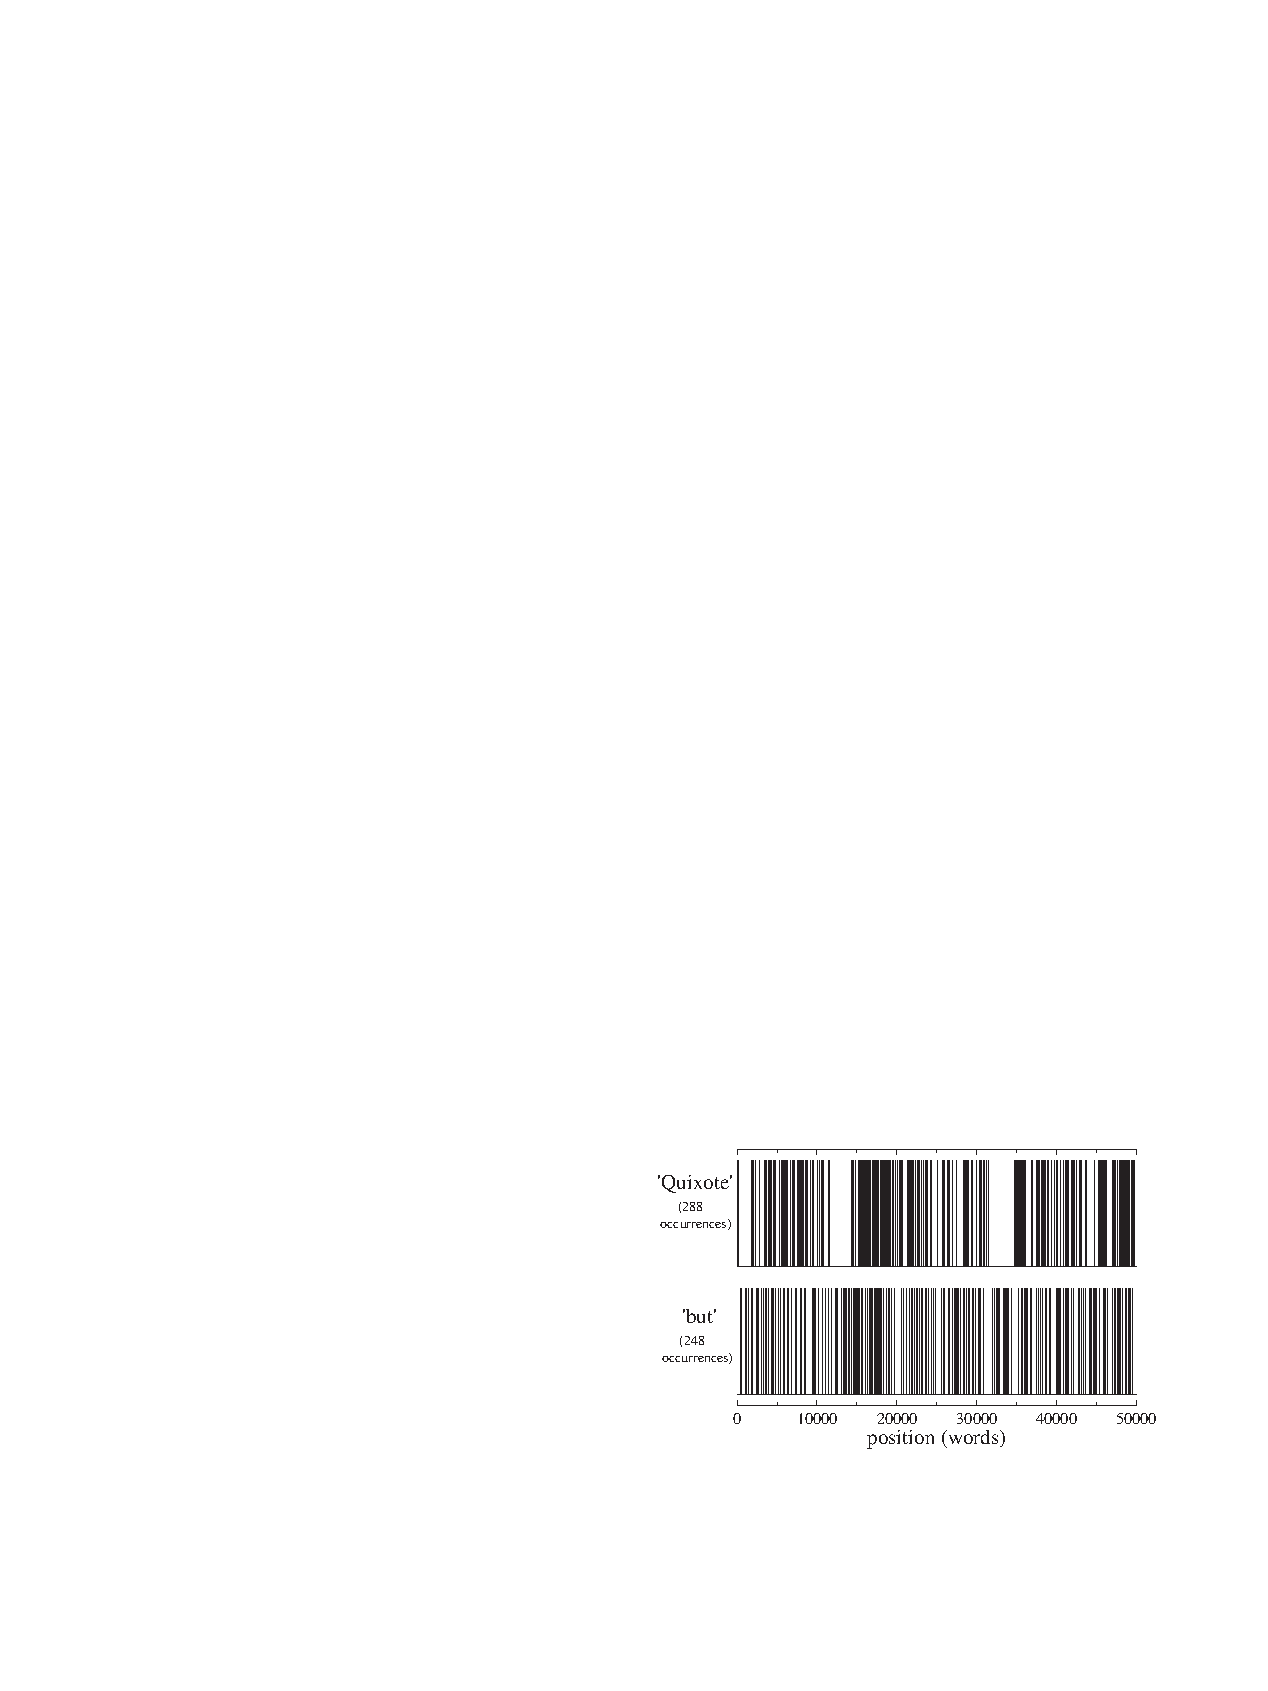
\includegraphics[width=.6\textwidth]{img/lit-survey/ols-keyword-spectra.pdf}
	\caption{Frequency spectra of `Quixote' (keyword, clustered distribution) and `but' (non-relevant, uniform distribution) in the first 50,000 words of \textit{Don Quixote}.}
	\label{fig:ols-spectra}
\end{figure}

This technique allows relevant keywords to be distinguished from non-relevant common words with similar total frequencies without the use of a background corpus for comparison.

Several important observations have been made regarding keyword extraction for news articles specifically. Firstly, that important phrases in text are likely to be references to people, places and other named entities \citep{NewsStand}. Libraries such as the Stanford Named Entity Recognizer (NER) \citep{NestedNamedEntityRecognition} exist to extract these from text. Secondly, while 30\% of an article's keywords are inferred and cannot be found within the text without intelligent input, 60\% are present in the article's title and first few sentences \citep{IdentifyingTopicsByPosition}, since important facts are generally stated as part of an article's \textit{above the fold} content.

%\subsection{Entity Disambiguation}

\section{The Metro Maps Metaphor}
Significant work in the area of information visualisation--and in particular, information \textit{cartography}--has been undertaken by Shahaf et al. \citep{ConnectingTheDots, GeneratingInformationMaps, MetroMapsOfScience, InformationCartographyPre}, in the domains of both news and science through the visualisation of article and journal data on metro maps.

The the metro map was introduced in \citep{GeneratingInformationMaps} to address the fact that previous timeline-based news summarisation systems could only represent simple linear stories; ``In contrast, complex stories display a very non-linear structure: stories split into branches, side stories, dead ends, and intertwining narratives.'' \citep[p.1]{InformationCartographyPre}

In this section, the formalisation of the metro map metaphor, its associated characteristics, and its limitations will be discussed.

\begin{definition}{Metro Map \citep{GeneratingInformationMaps}:}
A metro map $\mathcal{M}$ is a pair $(G, \Pi)$, where $G=(V, E)$ is a directed graph and $\Pi$ is a set of paths, or \textit{metro lines} in $G$. Each $e \in E$ must belong to at least one metro line.
\end{definition}

\begin{figure}[htbp!]
	\centering
	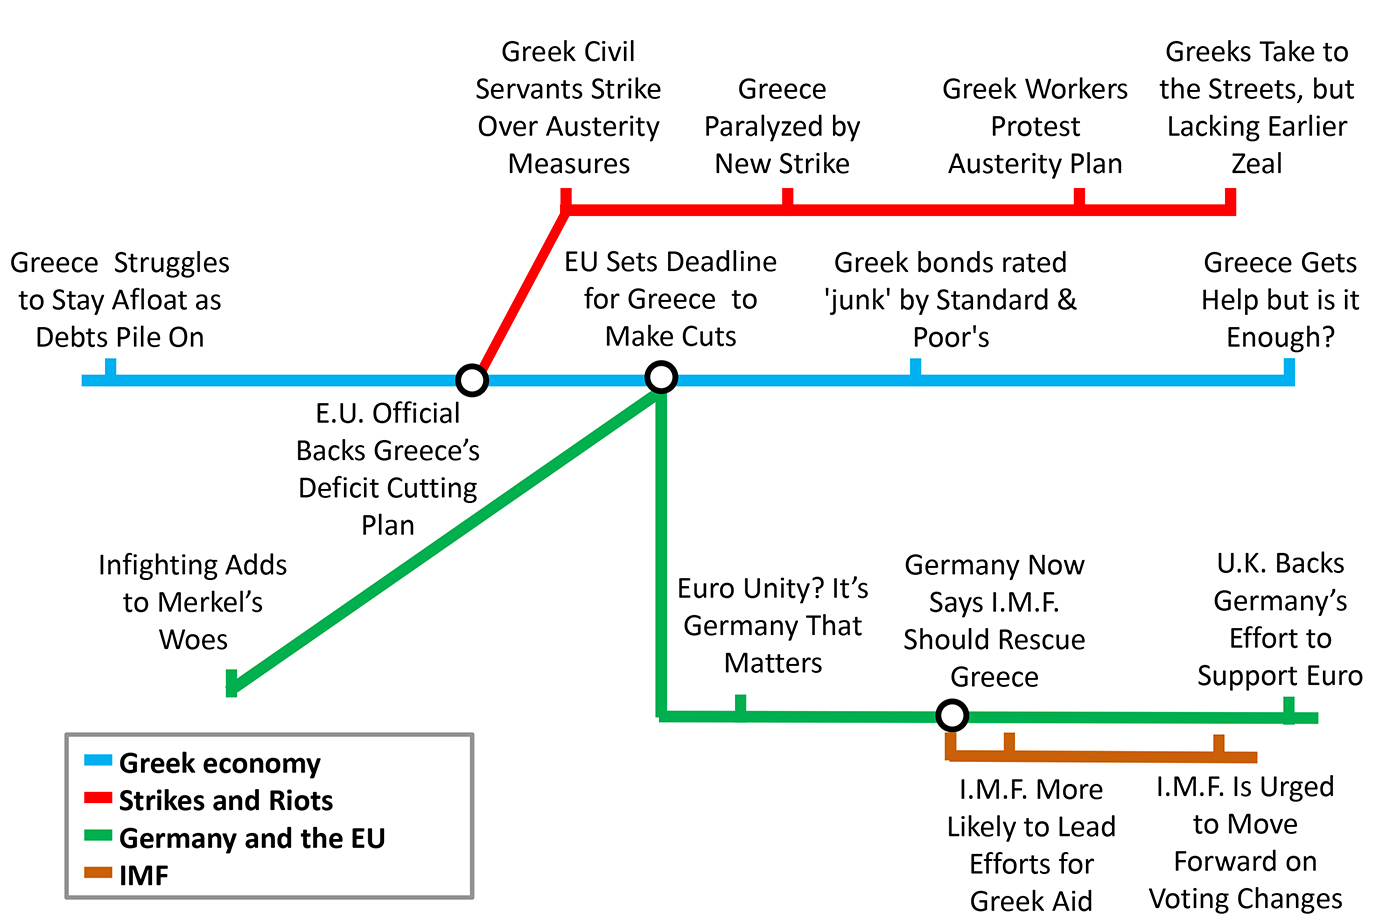
\includegraphics[width=.9\textwidth]{img/lit-survey/greece-metromap.jpg}
	\caption{A metro map \citep{GeneratingInformationMaps} covering the Greek Debt Crisis.}
	\label{fig:greecemetro}
\end{figure}

A previously published method \citep{ConnectingTheDots} for linking together chains of articles  was discussed, and an objective function was created to formalise the characteristics of a `good' metro map. The function defined was a composite based on three important characteristics, all of which are broadly applicable to the visualisation of any similar corpora; coherence, coverage, and connectivity.

\subsection{Coherence}
Let $\mathcal{D}$ be a set of articles, and $\mathcal{W}$ be a set of words or phrases, such that each article is a subset of $\mathcal{W}$. A \textit{coherent} chain of articles through $\mathcal{D}$ is one where transitions between documents are smoothed by common overlapping keywords from $\mathcal{W}$, creating a better narrative flow \citep{ConnectingTheDots} as depicted in Figure \ref{fig:coverage}.

\begin{figure}[htbp!]
	\centering
	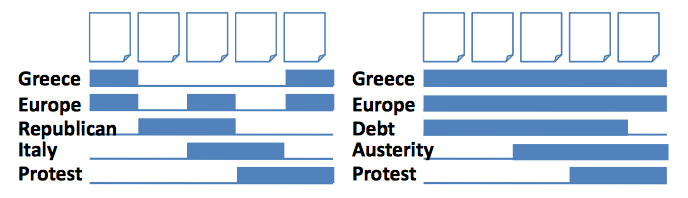
\includegraphics[width=.7\textwidth]{img/lit-survey/coverage.png} \par
	 \scriptsize{A bar corresponds to the presence of a word in the article above it.\\The titles of the articles which made up the two chains were as follows:\\[0.2cm]
	 \begin{tabular}{|l|l|}
	 	\hline 
	 	Chain A (left) & Chain B (right) \\
	 	\hline
	 	Europe weighs possibility of debt default in Greece & Europe weighs possibility of debt default in Greece \\
	 	Why Republicans don't fear a debt default & Europe commits to action on Greek debt \\
	 	Italy; The Pope's leaning toward Republican ideas & Europe union moves towards a bailout of Greece \\
	 	Italian-American groups protest `Sopranos' & Greece set to release austerity plan \\
	 	Greek workers protest austerity plan & Greek workers protest austerity plan \\
	 	\hline
	 \end{tabular}\vspace{0.2cm}}
	 \caption{An incoherent chain with jittery transitions between topics (Chain A, left) alongside a more coherent chain of articles (Chain B, right). \citep{GeneratingInformationMaps}}
	\label{fig:coverage}
\end{figure}

Coherence, intuitively, seems to be closely linked to idea of story resolution detailed in Section \ref{sec:information-overload}. This presents a question which could later be explored further; does forming coherent chains of articles provide the story resolution that participants in the Associated Press study were so desperately seeking from current events journalism?
	
\subsection{Coverage}
As in the previous section, let $\mathcal{D}$ be a set of articles, and $\mathcal{W}$ be a set of words or phrases of which the articles are composed. The coverage function for a word in a given document $d_i \in \mathcal{D}$ specified in Equation \ref{eqn:doc-coverage} can be quantified using any measure of how well $d_i$ covers $w$, for example TF-IDF$(w, d_i, \mathcal{D})$ (See Equation \ref{eqn:tfidf}) \citep{GeneratingInformationMaps}.
\begin{equation}
	\label{eqn:doc-coverage}
	cover_{d_i}(w) : \mathcal{W} \rightarrow [0,1]
\end{equation}
Extending the notion of coverage to maps--which can be abstracted to sets of documents--introduces the idea of \textit{diversity}. If a map already contains documents which for a sufficient coverage for some word $w$, then there is nothing to be gained by adding another document to $\mathcal{D}$ which has high coverage of $w$ alone. This relates back to the principles of spatial and information quality discussed in Section \ref{sec:information-overload}, especially the importance of value-added by every individual document in a collection. In this case, maps which cover a maximal number of $w \in \mathcal{W}$ should be preferential. A simple additive definition for map coverage such as Equation \ref{eqn:additive-coverage} \citep{GeneratingInformationMaps} would not reward this kind of diversity;
\begin{equation}
	\label{eqn:additive-coverage}
	cover_\mathcal{M}(w) = \sum_{d_i\in docs(\mathcal{M})}cover_{d_i}(w)
\end{equation}
Therefore, an alternative definition for map coverage was chosen, which will not increase significantly if another document which covers an already covered feature is added to $\mathcal{D}$ (Equation \ref{eqn:multiplicative-coverage} \citep{GeneratingInformationMaps}).
\begin{equation}
	\label{eqn:multiplicative-coverage}
	cover_\mathcal{M}(w) = 1 - \prod_{d_i\in docs(\mathcal{M})}(1-cover_{d_i}(w))
\end{equation}
Finally, the definition of map coverage is extended to the coverage of the corpus $\mathcal{D}$, rather than just single features. If each feature is weighted, according to frequency, then for each $w \in \mathcal{W}$ we have some $\lambda_w$. The coverage of a corpus $\mathcal{D}$ by a metro map $\mathcal{M}$ can then be defined as in Equation \ref{eqn:map-coverage} \citep{GeneratingInformationMaps}.
\begin{equation}
	\label{eqn:map-coverage}
	Cover(\mathcal{M}, \mathcal{D}) = \sum_{w \in \mathcal{W}}\lambda_w cover_\mathcal{M}(w)
\end{equation}

\subsection{Connectivity}
The final property is the most simply defined; the connectivity of a metro map is the number of paths in $\Pi$ which intersect \citep{GeneratingInformationMaps}.
\begin{equation}
	Connectivity(\mathcal{M}) = \sum_{i<j}\mathbbm{1}(p_i \cap p_j \neq\emptyset)
\end{equation}

\subsection{Limitations of \citep{GeneratingInformationMaps, InformationCartographyPre}}

\subsubsection{Corpus}
Perhaps the biggest limitation of the system developed in \citep{GeneratingInformationMaps, InformationCartographyPre} is the nature of the corpus $\mathcal{D}$; it is a fixed dataset, meaning users can only query it for certain non-recent events with no way of specifying a different corpus themselves. 

From a historical reference perspective the output provided for certain queries is interesting, but it is not possible to use the system as a replacement to a news feed aggregator or similar.

\subsubsection{Transit Map Aesthetics}
\todo{Write this}

\section{Evaluation Methods}
\citet{GeneratingInformationMaps} evaluated their system both for accuracy and with a user study. The accuracy evaluation tested whether the system included the most `important' (as decided by experts) documents in the map. The user study focused on the strength of the results returned by specific queries, where output was transformed into a structureless list in order for the study to be double-blind against the other methods. The evaluation was performed between-subjects, so background knowledge had to be controlled for. Output was compared with that from Google News and a TDT (Topic Detection and Tracking) method presented in \citep{SemanticLanguageModelsForTDT}. This approach to evaluation is less relevant to my proposed system, since it was actually evaluating the performance of the system in selecting documents based on a query, rather than visualising the documents on a map. In contrast, a visualisation and its usability is precisely the aspect of my process which I would ultimately need to evaluate.

\citet{EvaluatingInformationVisualisations} found that the evaluation of measures of usability such as task completion time and effectiveness can only be accurately conducted as part of a summative formal experiment. This is because formative tests such as think-aloud experiments require users to alter their behaviour and leads to slower actions \citep{VerbalReportsAsData}.

The evaluation of TIARA \citep{InteractiveTopicBasedVisualTextSummarizationAndAnalysis} was a more relevant method than the Metro Map evaluation as it was conducted against a baseline system which did not share any of its advanced features, although it was tailored for the same task; email analysis. A series of questions were asked of participants, who used either TIARA or the baseline system to answer. The response time and accuracy of the participants was recorded, as well as their levels of satisfaction after completing the task. This evaluation used between-subjects designs and therefore required the use of a different dataset for each task, as the nature of the sensemaking means any repetition of the evaluation task on the same data would see participants' performance improve significantly due to recall alone.

\section{Summary}
In summary, this review began with an exploration of the issue of news overload using the findings of \citep{anewmodelfornews}, a field study conducted into the news consumption habits of young people. The findings of the study were then discussed, firstly in the context of four dimensions of information overload \citep{TowardsAnOptimalResolutionToInformationOverload, GuestEditorsIntroductionInformationOverload} and secondly in terms of how they relate to sensemaking; the cognitive process this project aims to support.

Information visualisation was identified as one common approach to both support sensemaking and reduce information overload, so various methods for visualising text-based documents and news articles specifically were presented and compared \citep{ESTHETE, ThemeRiver, InteractiveTopicBasedVisualTextSummarizationAndAnalysis, ExploringLongRunningNewsStoriesUsingWikipedia, Nreader} as well as methods for transforming news articles into feature vectors for visualisation, such as mining, entity recognition, and keyword extraction.

Lastly, the work of Shahaf et al. \citep{ConnectingTheDots, GeneratingInformationMaps, MetroMapsOfScience, InformationCartographyPre} which is particularly relevant to the aims and objectives of this project was discussed in detail, with an explanation of key concepts (\textit{coherence}, \textit{coverage} and \textit{complexity}) defined in \citep{GeneratingInformationMaps} which are applicable to all graph-based representations of document collections.

Conducting this research has resulted in a clear direction of focus and scope for my project, and an understanding of what I could contribute to the domain of visualisation-based solutions to information overload. My aim is to integrate user-specified news feeds into the approach outlined in \citep{GeneratingInformationMaps} to generate custom maps based on current events, with a richer interactive display format and the addition of other techniques for reducing information load such as removing subsumed articles from the model \citep{UtilizingPhraseSimilarityMeasures} and attempting to provide contextual background in the visualisation itself \citep{ExploringLongRunningNewsStoriesUsingWikipedia}.

The resultant system would be a news feed aggregator with graphically structured visual output, and to the best of my knowledge would be the first of its kind.  
